\documentclass[twocolumn,10pt]{article}
\usepackage[a4paper, top=1.0in, bottom=1.0in, left=0.85in, right=0.85in]{geometry}

\usepackage{graphicx}
\usepackage{algorithm}  
\usepackage{algorithmicx}  
\usepackage{algpseudocode}  
\usepackage{amsmath}
\usepackage{url}

\renewcommand{\algorithmicrequire}{\textbf{Input:}}  
\renewcommand{\algorithmicensure}{\textbf{Output:}}  
\graphicspath{{figure/}}

\begin{document}

\date{November 17th, 2016}

\title{\bf Grouper: A Group Finance Manager on Mobile Devices Using Untrusted Servers}

\author{
	Meng Li, 201620728  
	\\ Supervisor: Yasushi Shinjo
}

\maketitle

\section{Introduction}
Conventional mobile applications are based on a client-server mode. This requires central servers for storing shared data. The users of such mobile applications must fully trust central servers and their application providers. Once this server is compromised by hackers, user information may be revealed because data is often stored on the server in cleartext. Finally, users may lose their data when service providers shut down their services. 

A group finance manager is an application that records the income and expenditure of a small group. A popular proposal is using P2P(Peer to Peer) to transfer user data between devices. However, there is a obvious problem in such a P2P proposal. Data transfer can only be finished during two devices are online at the same time. Another problem is that the number of P2P connections becomes large  fast as the number of users' increment.  In this paper, we are implementing without on trusted central servers. This means user data cannot be cracked easily and its data can be recovered from their own mobile devices. 

Unlike P2P systems, we use multiple untrusted servers for data transfer. Data is divided into several pieces and uploaded to diverse servers. Each server can only keep a piece of data temporarily. A piece will be deleted after a period of time. Those two methods ensure that user data cannot be cracked easily. In addition, all devices of group members keep a complete data set, data can be recovered even untrusted servers shut down.

\section{Design}

We design a group finance manager application, Grouper, on mobile devices. This does not rely on trusted central servers. 

\subsection{Group Finance Manager}
 In Grouper, group members generate records about money, classifications, accounts, shops, remark and times in their devices. For example, Alice records that she ate breakfast(classification) in center canteen(shop) at 8:00 AM(time) on November 1st, 2016, and she paid her breakfast by credit card(account). Of course, these classifications, shops and accounts are created by users as they want. They just select them when they want to add a new record.

 With data synchronization, they can also share their records with other group members, so that group income and expenditure information are analyzed and shown to all members. Grouper uses multiple untrusted servers to synchronize and avoids relying on trusted central servers. To create a group in Grouper, the owner of this group needs to register and set an access key in untrusted servers. The owner passes the access key to group members by a face-to-face way.

\subsection{Shamir's Secret Sharing}
In grouper, secret sharing plays an indispensable role in protecting user data from getting lost or destroyed. In a secret sharing scheme, a dealer securely shares a secret with a group of participants, by generating $n$ shares using a cryptographic function\cite{smith2013layered}. At least $k$ or more participants can reconstruct the secret, but $k-1$ or fewer participants can obtain nothing about the secret\cite{pang2005new}. We describe this scheme as a function $f(k, n)$, where n is the number of all shares, and k is the threshold to combine shares.  Shamir's Secret Sharing is a popular technique to implement threshold schemes.

\subsection{Data Synchronization Using Multiple Untrusted Servers}

We design Grouper based on data synchronization by multiple untrusted servers rather than a single server. There are three principles in our proposal. 

Firstly, a server transfers data as similar to a router, but does not keep it permanently. Most current popular client-server applications store user data on several central servers, and a user's data will not be deleted unless the user deletes his account. Grouper uses untrusted servers as a bridge for transferring data. Consider that a group includes three members: Alice, Bob and Carol. Alice creates a new record in her device, this record is uploaded to untrusted servers, and the record on servers will be eliminated after Bob and Carol download it from servers.

Secondly, a server keeps data temporarily. We define a period of time in which data can be kept in a server. In this paper, we set this period to 1 hour for our example situations. The record Alice uploaded to untrusted servers can only exist for 1 hour. After 1 hour since uploaded, this record will be deleted. Alice requires to upload this record again to serves until all of other members has downloaded successfully. The longer keeping period means the higher risk of data reveal. The most suitable period is influenced by the number of group members, security requirement and others. 

Thirdly, servers do not know the cleartext of data. Keeping data temporarily cannot ensure data security, because servers know the cleartext of data in this temporary period. For this problem, developers often encrypt data before uploading to servers, and this needs a decryption key to decrypt data in other devices. In order to distribute the decryption key, users should share it by themselves.

\begin{figure}[t]
\centering
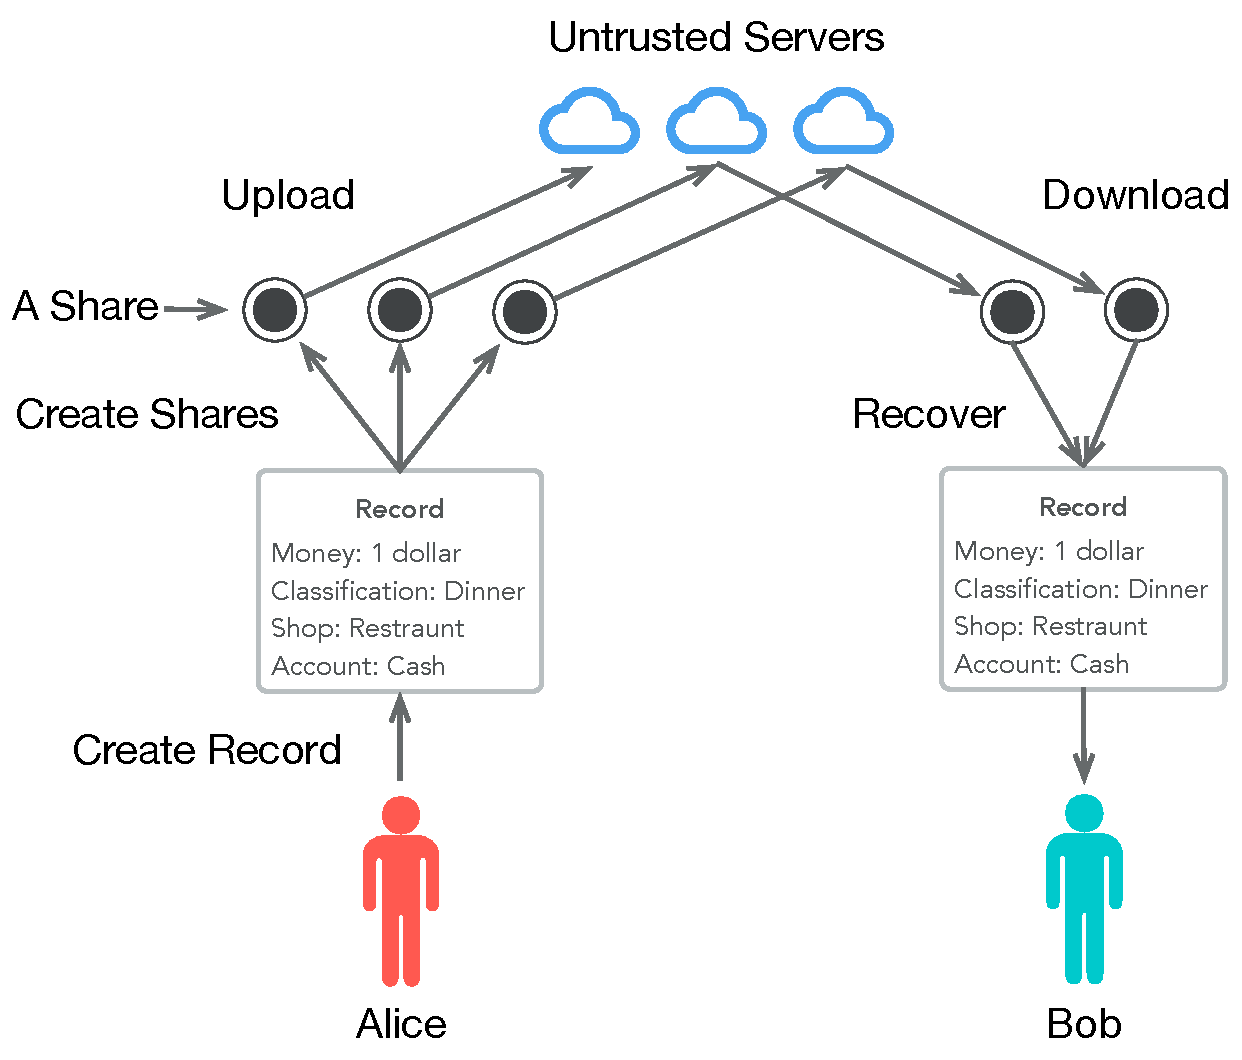
\includegraphics[scale=0.35]{sync_flow}
\caption{Flow of Synchronization}
\end{figure}

Figure 1 describes our synchronization flow based on these three principles. At first, Alice adds a record and Grouper creates a number of shares by secret sharing. Next, Grouper uploads those shares to multiple untrusted servers. When Bob is online, Grouper in Bob's device downloads shares from servers and recovers the new record created by Alice. In this situation, Grouper can recover the record after getting more than two shares. In this process, each server is separated from other servers, and cannot access to other servers. This means these servers cannot recover user data because they do not have permission to access other untrusted servers. In our proposal, only group members have permission to access these untrusted servers.

\subsection{Reliable Synchronization}
Grouper should provide a reliable synchronization service. For example, once Alice, who is a user in a group, creates a new record in her device, all of other members in a group should synchronize this record, even if this record may be deleted by untrusted servers after a period of time. We call this problem \emph{Reliable Synchronization}.

Figure 2 describes a unreliable situation that data cannot be synchronized. Alice sends a new record to untrusted servers at 10:00 AM and Bob downloads it successfully at 10:30 AM. Carol downloads failed after 11:00 AM because the shares of this record has been deleted by servers. To solve this problem, Alice should upload her new record again until Carol downloads it successfully. However, it is hard for Alice to get the information that all of other members in her group have download. We must find an efficient way for notifying Alice that all members have synchronized successfully.

\begin{figure}[t]
	\centering
	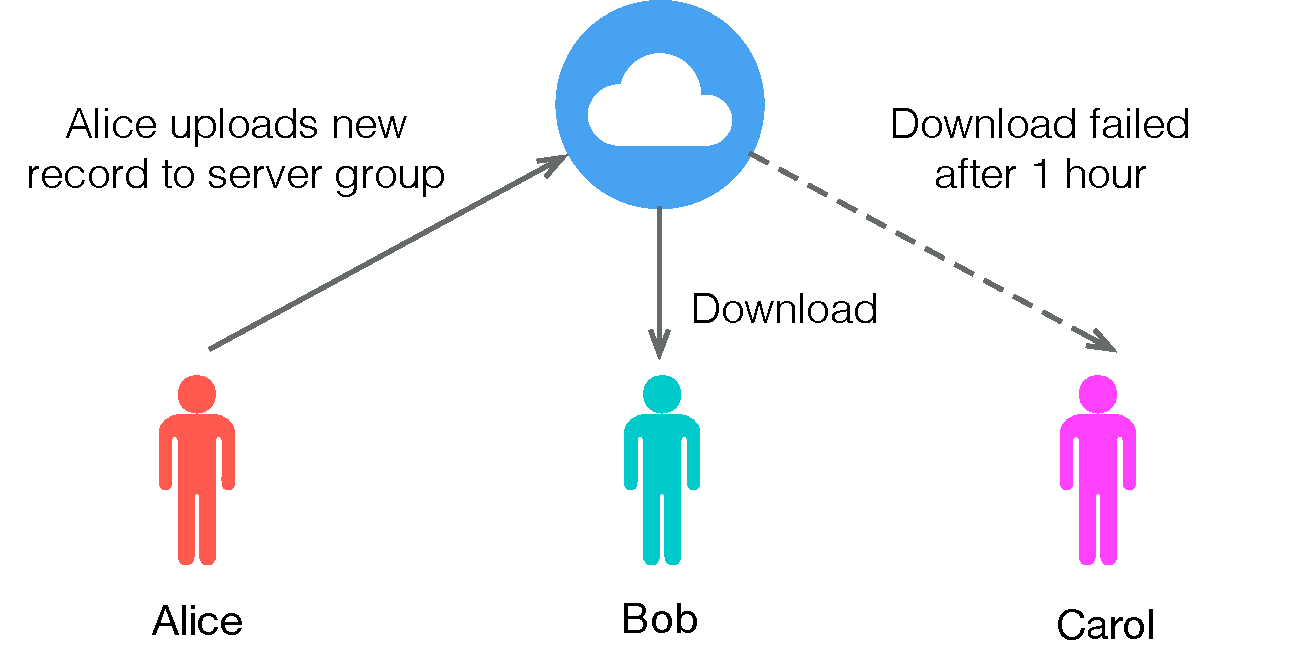
\includegraphics[scale=0.35]{unreliabe_sync}
	\caption{Unreliable Synchronization}
\end{figure}

If we consider a further problem that Carol, who is offline, can attack this group by being lazy. Alice, the record creator, has to upload shares to untrusted servers indefinitely. We are addressing this problem now by holding a list group members in untrusted servers.

\subsection{Create A Group}

A group in Grouper is created by its owner. For Alice, a group owner, she registers her group in three different untrusted server by submitting her own user information, group ID and group name. Here, user information is got from Facebook by OAuth. Group ID and group name is assigned by Alice and they should be same in all untrusted servers of this group. If there is no group same with Alice's new group in this untrusted server, Web service creates this new group successfully and return an access key generated by UUID including the highest privilege for Alice.

In Figure 3, we can see the procedure to add a new member to a group. At first, when Bob wants to join Alice's group, he will connect to Alice by a face-to-face way using Multipeer Connectivity framework. After establishing a connection between Alice and Bob, Bob will send his user information to Alice at first. Alice create a new user called Bob in three untrusted server of her group. Servers will return access keys for Bob to Alice. At last, Alice send access keys and user information to Bob, so that he can access to those untrusted server.

\begin{figure}[t]
	\centering
	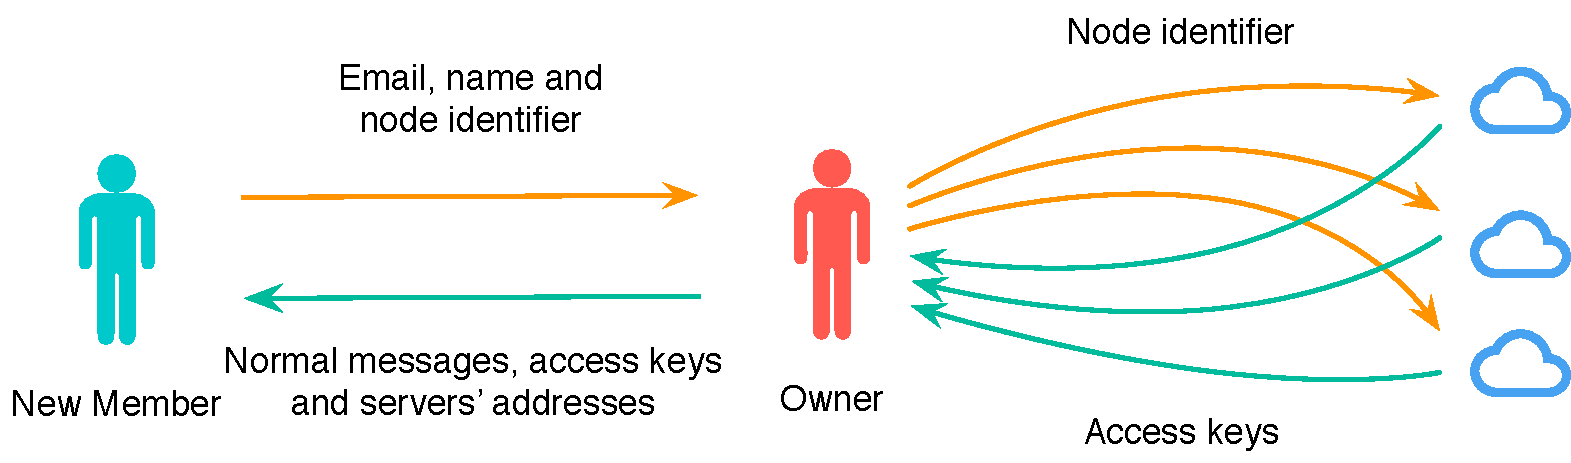
\includegraphics[scale=0.35]{add_member}
	\caption{Add New Member}
\end{figure}

\section{Implementation}
Grouper consists of client that run an iOS application and multiple untrusted servers run a Web service. In Section 2, we have introduced how to sharing a string with other deices via multiple untrusted servers. In this section, we describe persistent store and data synchronization. Grouper stores all data on mobile devices with an object-oriented way.

\subsection{Client}
 Grouper uses Core Data\cite{coredata}, a native iOS framework to manage the model layer objects. Core Data provides generalized and automated solutions to common tasks associated with object life cycle and object graph management, including persistence. Sync\cite{sync} by Elvis Nu\~{n}ez is a modern JSON synchronization framework to Core Data, and helps data synchronization parsing a JSON string. With Sync based on Core Data, we can concentrate on sharing with untrusted servers rather than data storage and synchronization.

In this paper, we use c-SSS\cite{c-sss}, an implementation of Shamir's Secret Sharing in C language by Fletcher T. Penney. This implementation supports UTF-8 character set without limitation of length. It provides two main functions: \emph{generate}, which generates $n$ shares by the string text with the threshold $k$, and \emph{extract}, which recreates the text string from more than $k$ shares. 

c-SSS generates shares from a JSON string. There shares are stored as an entity in Core Data. Grouper generates shares and upload them by a REST API to servers.

Figure 4 described the architecture of client. With untrusted untrusted servers, Grouper have to storage all data on mobile devices with an object-oriented way. Grouper use Core Data to storage and operate data as object. \emph{NSManagedObject+HYPPropertyMapper}, a part of Sync framework creates JSON string from object, and Sync synchronizes by parsing JSON String. c-SSS generates shares by JSON string and recover them to JSON string. REST API provided by web service in untrusted servers, controls data transferring between clients and servers. User information and server information are transferred between clients using Multipeer Connectivity framework by a face-to-face way.

Figure 5 is a screen shoot of the view \emph{Add Record}, users add a new record including money, classification, account, shop, time and remark in this view.

\begin{figure}[t]
	\centering
	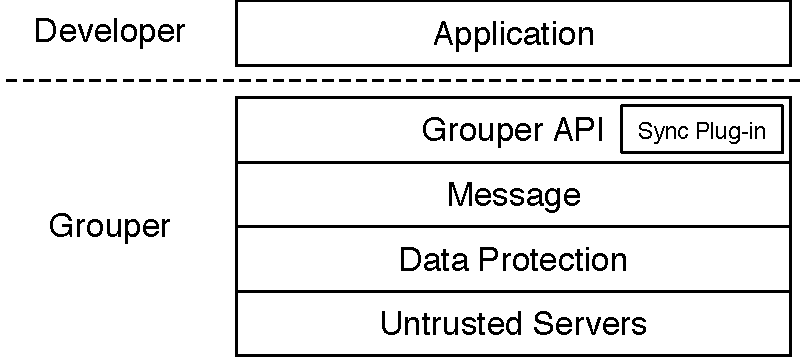
\includegraphics[scale=0.35]{architecture}
	\caption{Architecture of Client}
\end{figure}

\begin{figure}[t]
	\centering
	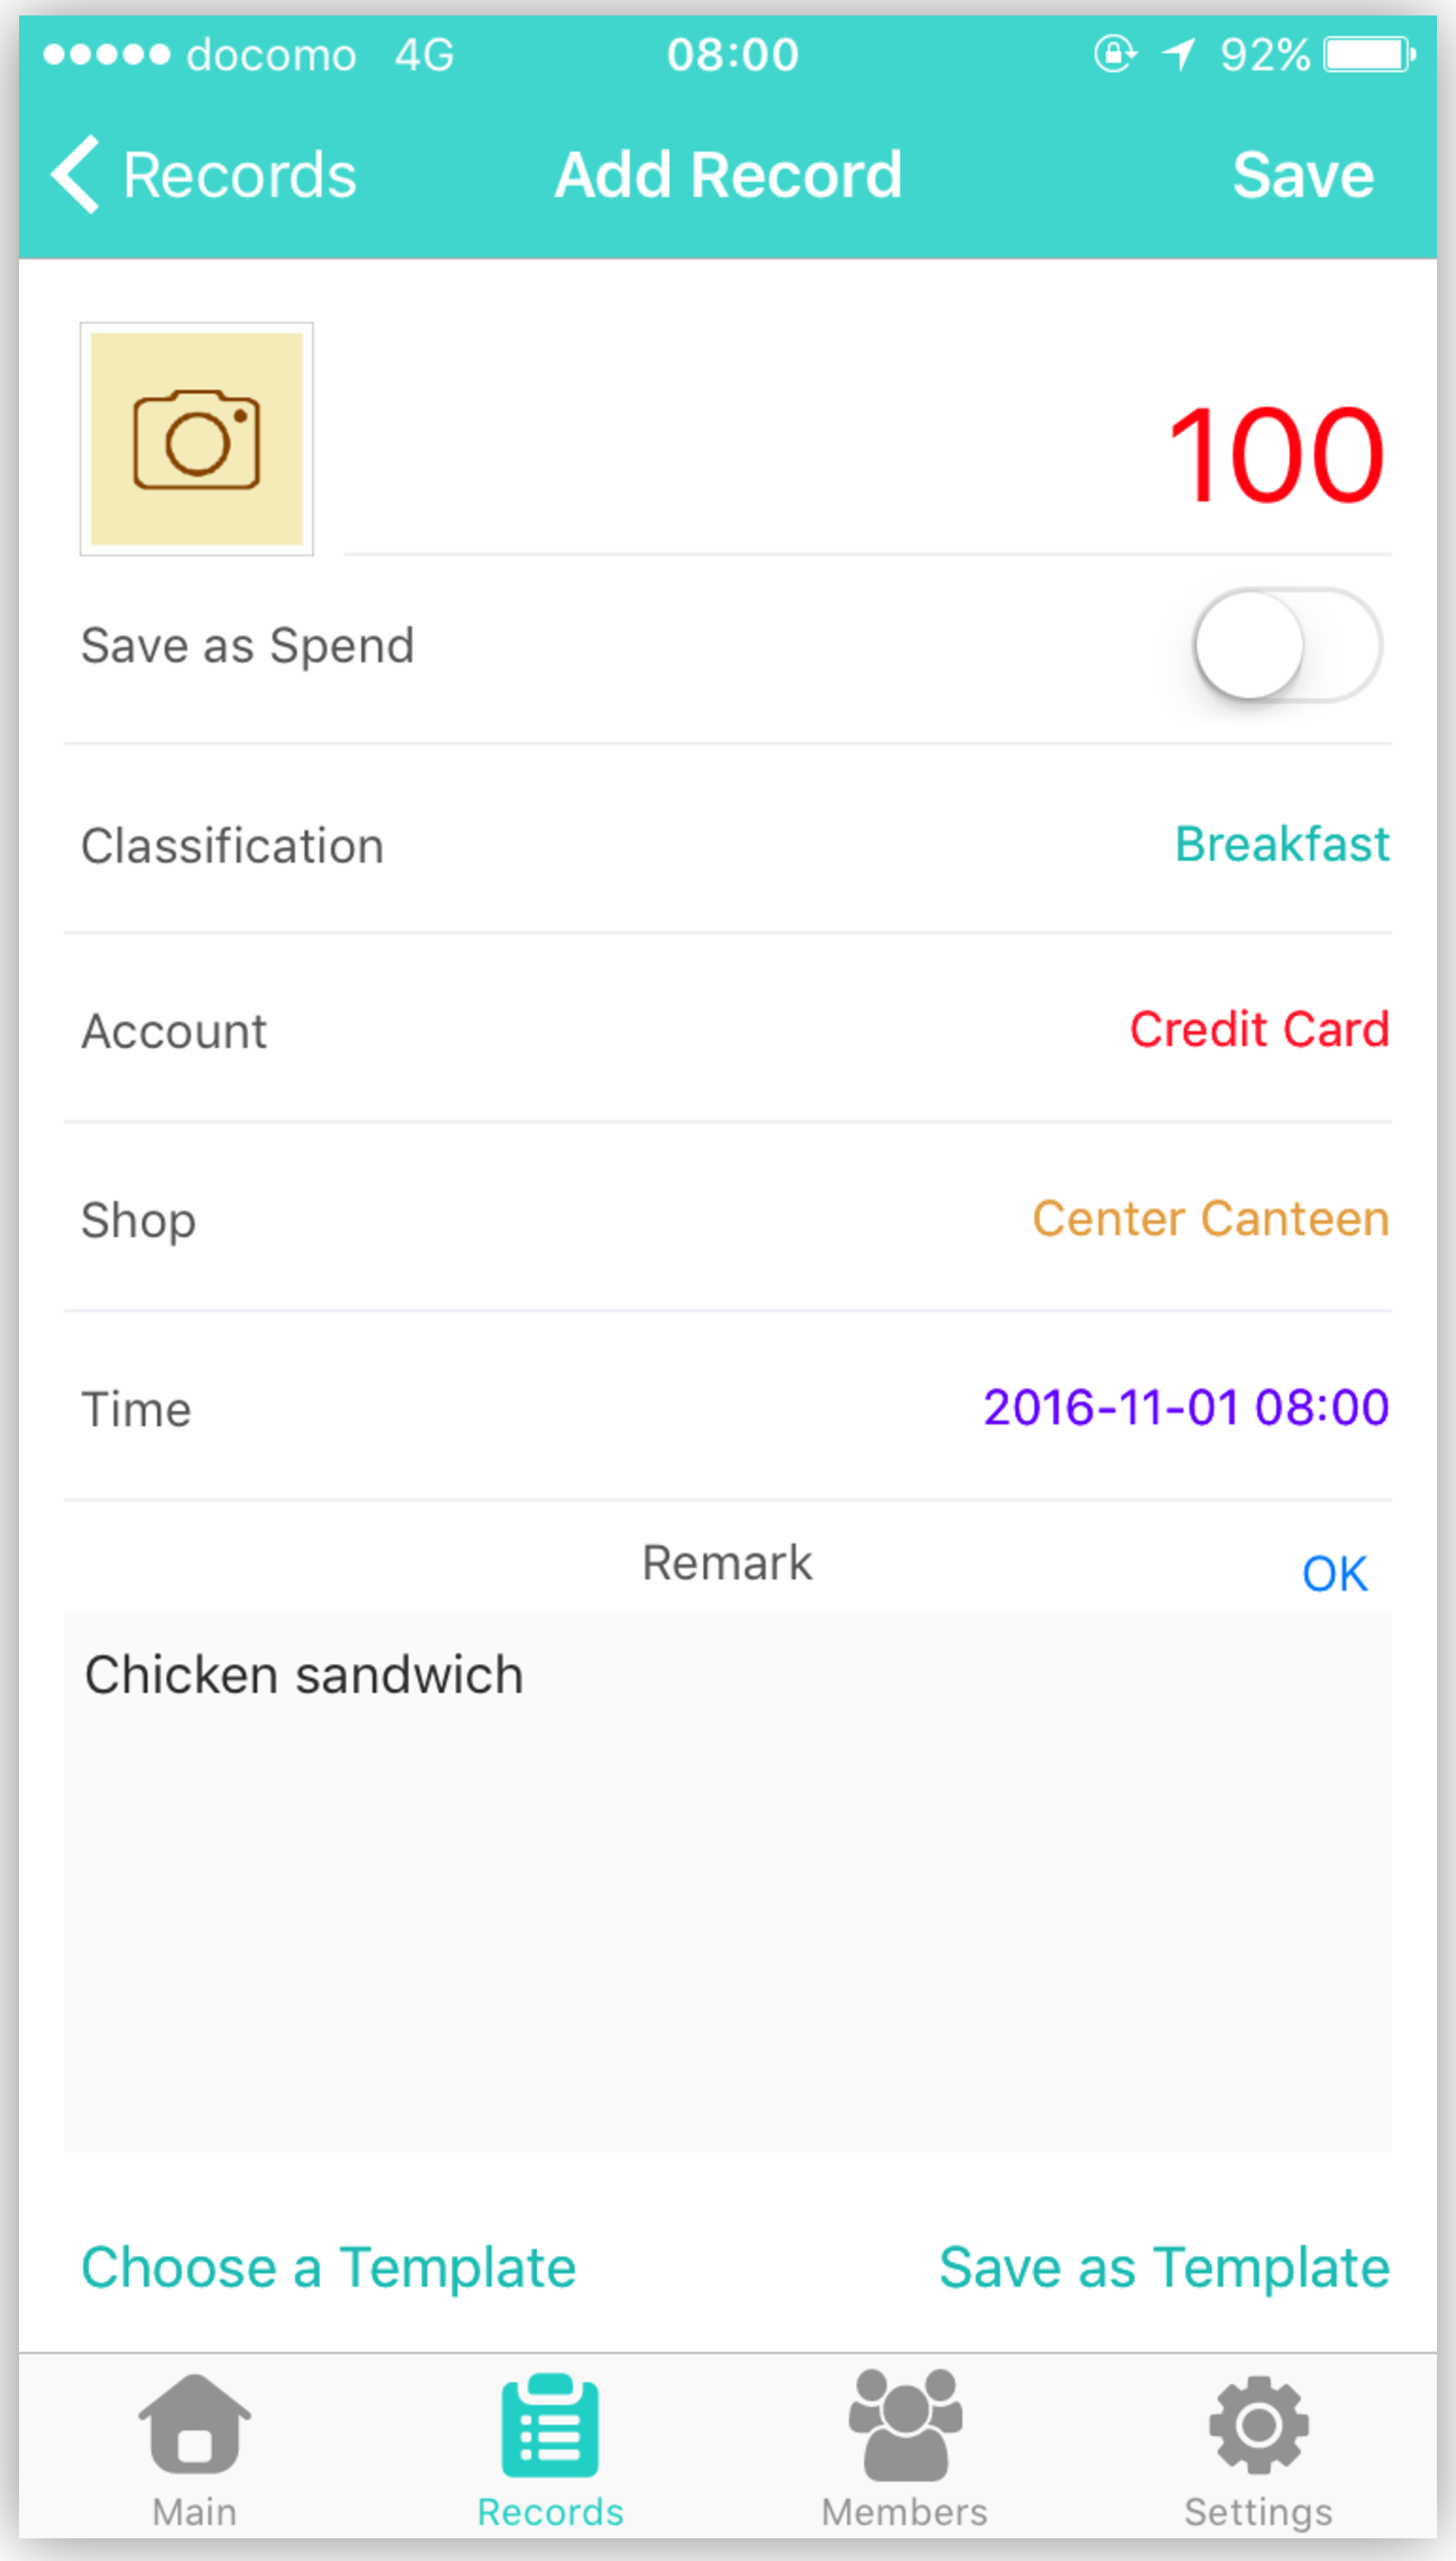
\includegraphics[scale=0.19]{screenshoot}
	\caption{Add Record Screen Shoot}
\end{figure}

\subsection{Web Service}
Many applications with synchronization use commercial cloud services like Amazon S3, Google Cloud and others. Grouper needs its own Web service rather than using commercial general cloud services for following reasons:

\begin{itemize}
\setlength{\itemsep}{1pt}
\setlength{\parskip}{0pt}
\setlength{\parsep}{0pt}
	\item The Web service should supports reliable synchronization.
    \item The Web service should ensure that shares are deleted after a prescriptive time.
    \item Only group members who has an access key can download shares from servers. In other word, a Web service plays a role of access control.
\end{itemize}

Our Web service runs on Tomcat server that is an open source implementation of the Java Servlet, JavaServer Pages, Java Expression Language and Java WebSocket technologies. We use Spring Web model-view-controller (MVC) framework to create our RESTful API. Like client, we use Hibernate, an open source Java persistence framework project, to save and operate object in Web service. Hibernate enables developers to more easily write applications whose data outlives the application process.

There are three entities including \emph{Group}, \emph{User} and \emph{Transfer} in Web service. Figure 6 describe the attributes of each entity and relationship between them. The relationship between \emph{Transfer} and \emph{User} and the relationship bwtween \emph{User} and \emph{Group} are \emph{Many-to-One}. The \emph{Group} entity saves the unique identifier, group name and its owner. The \emph{User} entity saves basic information of a user, access key for this user,and group of this user. The \emph{Transfer} entity saves the share generated with secret sharing scheme, saving time and its uploader. For each user, there is a unique access key for him in an untrusted server. This ensures that only he can remove or modify what he uploaded to this server. For a group, one of a user is its owner who has all the privileges of this group.

\begin{figure}[t]
	\centering
	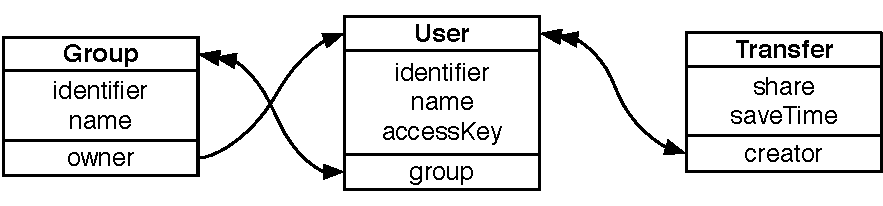
\includegraphics[scale=0.5]{entites}
	\caption{Entities in Web Service}
\end{figure}

\section{Related Work}

DepSky\cite{bessani2013depsky} is a system that stores encrypted data on servers and runs application logic on the client-side. DepSky provides a storage service that improves the availability and confidentiality by using commercial storage cloud services. \emph{Cloud-of-Clouds} is the core concept in DepSky. It represents that DepSky is a virtual storage cloud, and its users invoke operations in several individual severs. DepSky keeps encrypted data in commercial storage cloud services and do application logic in individual servers. In Grouper,  untrusted servers undertake responsibility of temporarily data storage and message delivery with server-side computation.

Mylar\cite{popa2014building} stores encrypted and sensitive data on a server, and decrypts this data only in users’ browsers. Developers of Mylar use its API to encrypt a regular(non-encrypted) Web application, and users decrypt data by a browser extension. Like Grouper, applications in Mylar can control how user data is shared. Mylar builds its system on a browser with browser extension while Grouper uses mobile device.

There are many applications or frameworks that use untrusted network and servers. Compared to them, Grouper uses secret sharing and temporary data storage with untrusted servers to protect user data from malicious attacking. Using secret sharing is more convenient and faster than using data encryption because clients need not to generate and share decryption key.

\section{Conclusion}

This paper introduces Grouper, a group finance manager that synchronizes data among mobile devices with multiple untrusted servers. Grouper uses Secret Sharing and temporary data storage services. Grouper consists of client that run an iOS application and multiple untrusted servers run a Web service. Each server of Grouper does not know the others and keeps one piece of the shares generated by secret sharing temporarily, to ensure that user data cannot be cracked easily. We are developing an application running in a iOS device and a Web service running on servers. We connect these clients and multiple untrusted servers by REST API.

\bibliographystyle{unsrt}
{
	\footnotesize
	\bibliography{ref}
}

\end{document}
